\chapter{Phase, Polarization, and Unitary Evolution}

This lecture begins by clearing up unfinished business about photon polarization, but it does not stay there. Leonard Susskind uses the two-state polarization system to sharpen three larger ideas: what we actually do with state vectors, why an overall phase has no physical meaning, and why time evolution must preserve inner products. What looks at first like a quick recap turns out to be the bridge from concrete polarization experiments to the formal language of Hermitian and unitary operators. These notes follow that lecture closely, with small board-based reconstructions supported by the preserved lecture frames; the original lecture is due to Leonard Susskind, and the supporting curation pipeline is credited to LazyingArt LLC and Video2Book.

\section{Polarization Observables Revisited}

The lecture opens by returning to the running example of photon polarization. The point is not merely to remind us of familiar matrices; it is to put a concrete two-state system back on the board before any more abstraction is introduced.

For horizontal and vertical polarization we take
\begin{equation}
\hat P_{xy}=
\begin{pmatrix}
1&0\\
0&-1
\end{pmatrix},
\qquad
|x\rangle=
\begin{pmatrix}
1\\
0
\end{pmatrix},
\qquad
|y\rangle=
\begin{pmatrix}
0\\
1
\end{pmatrix}.
\end{equation}
The operator $\hat P_{xy}$ has $|x\rangle$ and $|y\rangle$ as eigenvectors with eigenvalues $+1$ and $-1$. In the lecture this is read operationally: the two states are distinct outcomes of a polarization measurement.

For linear polarization at an angle $\theta$ we write
\begin{equation}
|\theta\rangle=
\begin{pmatrix}
\cos\theta\\
\sin\theta
\end{pmatrix}.
\end{equation}
An orthogonal partner can be chosen as
\begin{equation}
|\theta+\pi/2\rangle=
\begin{pmatrix}
\sin\theta\\
-\cos\theta
\end{pmatrix},
\end{equation}
or with the opposite overall sign. The lecture explicitly pauses to note that this sign choice does not matter physically; that observation will become important later.

The special $45^\circ$ states are therefore
\begin{equation}
|45^\circ,+\rangle=\frac{1}{\sqrt2}
\begin{pmatrix}
1\\
1
\end{pmatrix},
\qquad
|45^\circ,-\rangle=\frac{1}{\sqrt2}
\begin{pmatrix}
1\\
-1
\end{pmatrix},
\end{equation}
and the corresponding observable is the familiar
\begin{equation}
\hat P_{45}=
\begin{pmatrix}
0&1\\
1&0
\end{pmatrix}.
\end{equation}

The lecture then turns to circular polarization, where complex numbers make their first unavoidable appearance:
\begin{equation}
|C_+\rangle=\frac{1}{\sqrt2}
\begin{pmatrix}
1\\
i
\end{pmatrix},
\qquad
|C_-\rangle=\frac{1}{\sqrt2}
\begin{pmatrix}
1\\
-i
\end{pmatrix}.
\end{equation}
These are orthogonal provided we remember to complex conjugate in the inner product. The observable with these as eigenstates is
\begin{equation}
\hat P_{\mathrm{circ}}=
\begin{pmatrix}
0&-i\\
i&0
\end{pmatrix},
\qquad
\hat P_{\mathrm{circ}}|C_\pm\rangle=\pm |C_\pm\rangle.
\end{equation}

Already the lecture is making a physical point. Orthogonality is not being introduced as a sterile algebraic property. Two polarization states are orthogonal when one can be excluded with certainty in a single ideal measurement.

\section{What Quantum States Are For}

Having put the polarization example back in place, the lecture asks where this leaves us relative to the opening discussion of classical mechanics. Classically, a system with finitely many states is just a point in a finite set. An observable is then nothing but an assignment of numbers to those states. A coin may carry the values $\pm 1$ for heads and tails; a die already comes equipped with the labels $1,\dots,6$.

Quantum mechanics has gone one step farther. The state space is now a vector space, and observables are not mere labels but operators. At this stage Susskind narrows the discussion to the two physically interesting things we do with state vectors.

First, given a state $|\psi\rangle$ and an observable $\hat K$, we compute its expectation value:
\begin{equation}
\langle \hat K\rangle_\psi=\langle\psi|\hat K|\psi\rangle.
\end{equation}
This is the average we would obtain by preparing the same state repeatedly and measuring $K$ many times.

Second, if $|a\rangle$ and $|b\rangle$ are eigenvectors of two different observables,
\begin{equation}
\hat K|a\rangle=\alpha|a\rangle,
\qquad
\hat L|b\rangle=\beta|b\rangle,
\end{equation}
then the probability of preparing the system with definite $K=\alpha$ and later finding $L=\beta$ is
\begin{equation}
P(a\to b)=|\langle b|a\rangle|^2
=\langle a|b\rangle\langle b|a\rangle.
\end{equation}
The lecture emphasizes that the same expression also gives the reversed preparation-and-measurement order. At this level, these are the two basic quantum questions: ensemble averages and transition probabilities.

This is exactly the point at which the next conceptual move becomes possible. If two vectors are to represent the same physical state, then they must agree on expectation values and on transition probabilities.

\section{Overall Phase Has No Physical Meaning}

Before discussing phase, the lecture inserts a normalization rule. Physical state vectors are unit vectors:
\begin{equation}
\langle\psi|\psi\rangle=1.
\end{equation}
That fixes the total probability to be one. But even after normalization there remains another operation we can perform on the whole state: we may multiply it by a pure phase.

A complex number can be written as $z=re^{i\theta}$, and its complex conjugate is $z^*=re^{-i\theta}$. For a pure phase we have $r=1$, so
\begin{equation}
z=e^{i\theta},
\qquad
z^*=e^{-i\theta},
\qquad
zz^*=1.
\end{equation}
Geometrically these are the points on the unit circle in the complex plane.

\begin{figure}[t]
\centering

\includegraphics[width=0.72\textwidth]{lecture_07_figure_02.png}
\caption{Phase-related state vectors and the accompanying unit-circle sketch from the lecture board.}
\end{figure}

\begin{figure}[t]
\centering
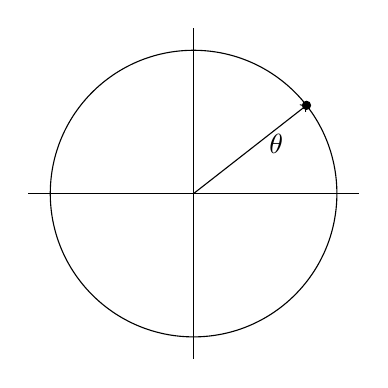
\begin{tikzpicture}[scale=1.4]
\draw (0,0) circle (1.3);
\draw (-1.5,0)--(1.5,0);
\draw (0,-1.5)--(0,1.5);
\draw[->] (0,0)--(38:1.3);
\fill (38:1.3) circle (1.2pt);
\node at (0.75,0.45) {$\theta$};
\end{tikzpicture}
\caption{Clean reconstruction of the phase-circle picture used to motivate the factor $e^{i\theta}$.}
\end{figure}

The board now compares two vectors:
\begin{equation}
|A\rangle,
\qquad
e^{i\theta}|A\rangle.
\end{equation}
Mathematically these are different vectors. The second is obtained by multiplying the first by a complex number. But the lecture insists that they have the same physical significance. The reason is not mysterious; it is immediate from the two things states are used for.

If we replace $|\psi\rangle$ by $e^{i\theta}|\psi\rangle$ in an expectation value, then
\begin{align}
\langle e^{i\theta}\psi|\hat K|e^{i\theta}\psi\rangle
&=
e^{-i\theta}e^{i\theta}\langle\psi|\hat K|\psi\rangle \\
&=
\langle\psi|\hat K|\psi\rangle.
\end{align}
The phase cancels between bra and ket.

The same happens for a transition probability. For example, if we multiply $|b\rangle$ by a phase,
\begin{align}
|\langle e^{i\theta}b|a\rangle|^2
&=
\langle a|e^{i\theta}b\rangle\langle e^{i\theta}b|a\rangle \\
&=
e^{i\theta}e^{-i\theta}\langle a|b\rangle\langle b|a\rangle \\
&=
|\langle b|a\rangle|^2.
\end{align}
Thus all expectation values and all transition probabilities are insensitive to the overall phase.

A simple example is already on the board:
\begin{equation}
|y\rangle=
\begin{pmatrix}
0\\
1
\end{pmatrix},
\qquad
-|y\rangle=
\begin{pmatrix}
0\\
-1
\end{pmatrix}.
\end{equation}
Multiplication by $-1$ is multiplication by the phase $e^{i\pi}$. The two vectors are not equal, but they describe the same physical polarization.

The same is true for circular polarization:
\begin{equation}
\frac{1}{\sqrt2}
\begin{pmatrix}
1\\
i
\end{pmatrix}
\qquad\text{and}\qquad
\frac{1}{\sqrt2}
\begin{pmatrix}
i\\
-1
\end{pmatrix}
\end{equation}
differ by the pure phase $i=e^{i\pi/2}$ and therefore represent the same physical state.

\subsection{Question \& Answer}

Why are $|\psi\rangle$ and $e^{i\theta}|\psi\rangle$ physically the same if they are mathematically different?

Because the lecture has already identified the physically meaningful questions. We ask for expectation values and for transition probabilities. Both depend on a state only through bra-ket sandwiches and squared overlaps, and in both cases an overall phase cancels against its complex conjugate. So the physical state is not a single nonzero vector but a whole phase-equivalence class of vectors.

\section{Counting the Parameters of Photon Polarization}

With phase indifference established, the lecture returns to photon polarization and asks how many parameters it really takes to describe a physical photon state.

We begin with a general two-component vector,
\begin{equation}
|\psi\rangle=
\begin{pmatrix}
\alpha\\
\beta
\end{pmatrix},
\end{equation}
where $\alpha$ and $\beta$ are complex numbers. That gives four real parameters. Normalization imposes one relation,
\begin{equation}
\alpha^*\alpha+\beta^*\beta=1,
\end{equation}
so we are down to three. Then overall phase removes one more degree of freedom.

The lecture phrases this concretely: by multiplying the whole vector by a suitable phase, we may always choose the upper entry to be real. Write it as $a\in\mathbb R$. Then
\begin{equation}
a^2+\beta^*\beta=1,
\end{equation}
so $|\beta|=\sqrt{1-a^2}$, and therefore
\begin{equation}
\beta=\sqrt{1-a^2}\,e^{i\phi}.
\end{equation}
The state can thus be written as
\begin{equation}
|\psi\rangle=
\begin{pmatrix}
a\\
\sqrt{1-a^2}\,e^{i\phi}
\end{pmatrix}.
\end{equation}

At this point the counting is complete:
\begin{enumerate}
\item two complex entries give four real parameters,
\item normalization removes one,
\item overall phase removes one more,
\item a physical photon polarization state therefore depends on two real parameters.
\end{enumerate}

The lecture also regularizes notation at this stage. The same symbol $\theta$ had been serving both as a linear-polarization angle and as a phase angle. To avoid collision, the relative phase is renamed $\phi$. That is a small but important repair to the story, and we keep it.

\section{From State Vectors to Elliptical Polarization Geometry}

The next move is characteristic of the lecture. We have counted two real parameters algebraically, and now we ask what those two parameters mean physically.

For a plane-polarized electromagnetic wave the electric field points along a single axis. If the wave is traveling into the board, then the polarization is specified by the direction of that axis. That is a one-parameter family.

If we superpose two linear polarizations in phase, the result is still plane polarization, merely along a different axis. But once the two components are out of phase, the tip of the electric field no longer moves on a line. It may sweep out a circle, and more generally an ellipse.

The lecture uses simple examples. If
\begin{align}
E_x&=\cos(x-ct),&
E_y&=\sin(x-ct),
\end{align}
then at fixed position, say $x=0$, the electric field rotates on a circle. This is circular polarization. If instead we reduce the second component, for example
\begin{equation}
E_y=\frac12\sin(x-ct),
\end{equation}
then at fixed $x$ the field traces an ellipse. In that example the major axis lies along the $x$ direction.

So the two physical parameters are read off geometrically:
\begin{enumerate}
\item the angle of the major axis,
\item the eccentricity, or more precisely in the lecture's language the aspect-ratio parameter of the ellipse.
\end{enumerate}

There are two useful limiting cases. When the ellipse collapses to a line, we recover plane polarization. When it becomes a circle, there is no distinguished major axis left. This is why circular polarization is a special case inside the general two-parameter family.

\begin{remark}
The lecture uses the word eccentricity loosely, more like the ratio of minor to major diameter than the standard textbook eccentricity. In that lecture language, the parameter runs from linearly polarized to circularly polarized and is then extended through zero to negative values to encode the opposite sense of rotation.
\end{remark}

\subsection{Question \& Answer}

Where did clockwise versus counterclockwise polarization go if there are only two real parameters?

The lecture's answer is that the handedness is not an extra parameter once we allow the ellipse parameter to pass through zero and become negative. Start from circular polarization, squeeze the circle into an ellipse, then squeeze it all the way down to a line. If one keeps going, the upper and lower branches exchange roles, and the sense of rotation reverses. In that heuristic but useful language, negative eccentricity encodes the opposite handedness. Thus two real parameters still suffice: angle and signed ellipse parameter.

\section{Overlap With Linear Polarization and the Major Axis}

Now the lecture asks a concrete question. Given a general elliptically polarized photon, how would we recover the direction of its major axis by measurement?

We compare the elliptic state with a linearly polarized state at analyzer angle $\theta$:
\begin{equation}
|\theta\rangle=
\begin{pmatrix}
\cos\theta\\
\sin\theta
\end{pmatrix},
\qquad
|\psi\rangle=
\begin{pmatrix}
a\\
\sqrt{1-a^2}\,e^{i\phi}
\end{pmatrix}.
\end{equation}

\begin{figure}[t]
\centering

\includegraphics[width=0.82\textwidth]{lecture_07_figure_03.png}
\caption{State-vector overlap and geometric sketches as laid out on the lecture boards.}
\end{figure}

The lecture writes the overlap and then corrects the phase by remembering that one factor must be conjugated. In cleaned form,
\begin{equation}
\langle\psi|\theta\rangle
=
a\cos\theta+\sqrt{1-a^2}\,e^{-i\phi}\sin\theta.
\end{equation}
The order of bra and ket is partly obscured on the board, but the conjugated phase in the final cleaned expression is secure from the spoken correction.

\begin{remark}
Here we deliberately keep the cleaned amplitude close to the lecture rather than presenting a fully polished textbook derivation. The board is partially occluded, and Susskind corrects the conjugation in real time.
\end{remark}

The transmission probability through a linear polarizer aligned at angle $\theta$ is then
\begin{equation}
P_\theta(\psi)=|\langle\psi|\theta\rangle|^2.
\end{equation}
This is not yet the full computation on the board. In fact the lecture explicitly refuses to carry the algebra to the end and assigns that step as homework. But the prescription is perfectly clear: hold $\phi$ fixed, square the modulus, and maximize with respect to $\theta$:
\begin{equation}
\frac{d}{d\theta}P_\theta(\psi)=0.
\end{equation}
The angle at which $P_\theta(\psi)$ is largest gives the direction of the major axis.

\begin{figure}[t]
\centering
\begin{tikzpicture}[scale=1.2]
\draw[->] (-2,0)--(2.2,0);
\draw[->] (0,-1.6)--(0,1.8);
\draw (0,0) ellipse (1.4 and 0.7);
\draw[dashed] (-1.6,-0.8)--(1.6,0.8);
\draw[thick] (-1.2,-0.6)--(1.2,0.6);
\node at (1.55,0.95) {$\theta$};
\end{tikzpicture}
\caption{A conservative reconstruction of the geometric idea: vary the analyzer direction until the overlap with the elliptic state is maximal.}
\end{figure}

The lecture says less about extracting the eccentricity. The suggestion is qualitative: compare probabilities along the major and minor directions, and their difference measures how asymmetric the ellipse is. Since the lecture does not push that computation further, we leave it at that level.

\section{Time Evolution, Hermitian Operators, and the Unitary Pivot}

The last long movement of the lecture leaves polarization as a static example and asks how states change with time. This is the real destination of the whole discussion.

\subsection{Relations Between States}

Classically, if the state space is a finite set of points, time evolution is a permutation of those points. Distinct initial states stay distinct. Otherwise information about the initial condition would be lost.

Quantum mechanics has a richer notion of relation between states. Two normalized states may be identical, orthogonal, or somewhere in between. Operationally, horizontal and vertical polarization give the sharp example: a vertically polarized photon will not pass a horizontal polarizer. Thus
\begin{equation}
\langle y|x\rangle=0
\end{equation}
expresses measurable orthogonality.

More generally, for normalized states,
\begin{equation}
\langle B|A\rangle=0
\end{equation}
means complete orthogonality, while
\begin{equation}
\langle B|A\rangle=1
\end{equation}
means the same state. Intermediate values measure partial overlap and therefore partial distinguishability.

The quantum analog of classical distinction-preservation is then immediate: as the system evolves, these overlaps are preserved. If
\begin{equation}
|A\rangle\to |A'\rangle,
\qquad
|B\rangle\to |B'\rangle,
\end{equation}
then
\begin{equation}
\langle B'|A'\rangle=\langle B|A\rangle.
\end{equation}
In particular, states that begin orthogonal remain orthogonal.

\subsection{Hermitian Conjugation And Observables}

After the break the lecture becomes more formal. Suppose $L$ is a linear operator acting on ket vectors. Its action on bra vectors is defined so that sandwiches can be interpreted consistently from either side. In a complete orthonormal basis,
\begin{equation}
\sum_n |n\rangle\langle n|=I.
\end{equation}
Matrix elements are written as
\begin{equation}
\langle n|L|m\rangle.
\end{equation}
The Hermitian conjugate is then defined by reversing bra and ket and complex conjugating:
\begin{equation}
\langle n|L^\dagger|m\rangle=\langle m|L|n\rangle^*,
\qquad
(L^\dagger)_{nm}=L_{mn}^*.
\end{equation}
So Hermitian conjugation is transpose plus complex conjugation.

An operator is Hermitian when
\begin{equation}
L=L^\dagger.
\end{equation}
In matrix language this means the diagonal entries are real,
\begin{equation}
L_{ii}=L_{ii}^*,
\end{equation}
and the off-diagonal entries are complex conjugates across the diagonal,
\begin{equation}
L_{ij}=(L_{ji})^*.
\end{equation}

The lecture returns for a moment to the polarization operators to check that they are indeed Hermitian:
\begin{equation}
\hat P_{xy}=
\begin{pmatrix}
1&0\\
0&-1
\end{pmatrix},
\qquad
\hat P_{45}=
\begin{pmatrix}
0&1\\
1&0
\end{pmatrix},
\qquad
\hat P_{\mathrm{circ}}=
\begin{pmatrix}
0&-i\\
i&0
\end{pmatrix}.
\end{equation}
Each has real diagonal entries, and each pair of off-diagonal entries are complex conjugates. These are therefore legitimate observables.

The lecture also states the standard equivalent characterization: Hermitian operators have complete orthonormal sets of eigenvectors with real eigenvalues. That is why observables are represented by Hermitian operators: the possible measured values are real, and the corresponding eigenstates span the space.

\subsection{Unitary Operators}

But observables are not yet time evolutions. Time evolution is a transformation of the vector space that preserves relations between states. Let $U$ be such a transformation:
\begin{equation}
U|A\rangle=|A'\rangle,
\qquad
U|B\rangle=|B'\rangle.
\end{equation}
The corresponding bras transform with $U^\dagger$:
\begin{equation}
\langle A'|=\langle A|U^\dagger,
\qquad
\langle B'|=\langle B|U^\dagger.
\end{equation}
Now impose preservation of inner products:
\begin{align}
\langle B'|A'\rangle
&=
\langle B|U^\dagger U|A\rangle \\
&=
\langle B|A\rangle.
\end{align}
If this holds for every pair of states $|A\rangle$ and $|B\rangle$, then the operator between them must be the identity:
\begin{equation}
U^\dagger U=I.
\end{equation}
Equivalently,
\begin{equation}
U^\dagger=U^{-1}.
\end{equation}
That is the defining property of a unitary operator.

The lecture insists on the right physical reading. A unitary operator is not the identity operator; it may move vectors around the state space. But it moves them around in a way that preserves all the relationships that matter, namely the overlaps and therefore the probabilities. That is why unitary operators govern time evolution, and also why they represent symmetry operations.

The lecture closes by stating, rather than proving in detail, that unitary operators also possess complete orthonormal sets of eigenvectors. Their eigenvalues need not be real; the analysis of those eigenvalues is deferred to the next lecture, together with the introduction of Hamiltonians. The message at the end is already clear enough: systems change with time by unitary transformation.

\section{Summary}

This lecture begins with photon polarization and ends with the general structure of quantum time evolution. Along the way we learn that the physically meaningful content of a state-vector is carried not by the vector itself but by its phase-equivalence class, that a single-photon polarization state depends on two real parameters, and that those two parameters can be read geometrically as the orientation and shape of the polarization ellipse. Once the relation between states is recognized as the inner product, the final step follows almost inevitably: the transformations that preserve physics are the unitary ones, satisfying $U^\dagger U=I$. The next lecture will take that statement seriously and ask what such operators look like in time-dependent quantum mechanics.